\TitreIntro{Préface}

%\newline

% J'ai enlevé la lettrine car ca faisait pas beau. Si vous trouvez comment améliorer ca à vous de le changer!
%\begin{floatingfigure}[]{5mm}
%
\includegraphics[height=10mm]{intro/preface/img/lettrine-i.jpg}
%\end{floatingfigure}

Il arrive quoi dans un sous-sol démoralisant, anémiant et sale, lorsque des gens jusque-là prostrés, cloîtrés et gommés des registres, se mettent à vivre toute une gamme de sentiments humains, partant de vieilles blessures cachées bien creux qui s’ouvrent, passant par des décennies de non-dit, de colère refoulée et d’ambitions détruites, finissant dans les larmes, le sourire et le bonheur ? Il arrive quoi si ces gens sont âgés, désabusés, démunis et totalement dépendants de la bienveillance sans borne d’un fils persécuté qui, à 43 ans, est encore puceau et déteste jouer du trombone ? Que se passe-t-il quand ces gens se cachent d’un système qui traque et enferme les vieux dont certains se retrouvent intubés dans un projet de production hormonale ? Il arrive une histoire sordide où les méchants sont vraiment affreux, une histoire rocambolesque où les bons sont hauts en couleur, une histoire d’amour pleine de chaudes émotions sous fond de musique allemande, Wie einst Lili Marleen, une histoire de commando dont le colonel est l’arrière-petit-fils de l’inventeur du Pétépano et la générale, une joueuse de violoncelle..

\begin{floatingfigure}[r]{40mm}

\includegraphics[height=60mm]{intro/preface/img/hopital.jpg}
\end{floatingfigure}

Pourtant, l’idée de départ était bien différente. Elle était sensée répondre à mes craintes quant aux années à venir. Elle se basait sur un fait vécu, une anecdote déplaisante que j’avais à peine arrangée et qui avait pour cadre une salle d’urgence québécoise durant l’été 2008.La dame a son expression des grands jours, celle où c’est écrit «j’ai pas le temps de niaiser».

- Maman, ils m’ont dit de venir te chercher, qu’ils ne pouvaient plus te garder, qu’il me fallait te ramener à la maison.

Puis, pour elle-même, elle ajoute :

- Qu’il fallait qu’à 57 ans, j’apprenne à être ton «aidant naturel».

La vieillarde décoiffée et édentée lève un peu la tête de sa civière. De ses yeux creux, elle regarde cette femme en larmes qui la dévisage de si près. Elle ne comprend pas et se retourne vers le mur. Derrière elle, devant elle, d’autres civières. Des cancers, des poumons, des boyaux, des os, des enflures, des cirrhoses. Ça sent le cabinet d’aisance achalandé. Il fait chaud à vomir. Ça geint, ça craint, ça ne veut pas être seul, ça veut savoir. Sans arrêt, des hommes et des femmes en uniforme d’hôpital passent, toujours à la course, toujours pour d’autres, toujours avec d’autres priorités, toujours sans les regarder. Des ambulanciers vont et viennent des dossiers en main. Des bonhommes promènent leur verre de styromousse plein de café de machine, d’autres essaient de regarder une télé pas de son qu’on a boulonnée trop haut pour être vue sans torticolis, d’autres se sont ramassé le Journal de Québec et, après les petites annonces, en sont rendus à lire les avis de décès non sans quelque espoir de pouvoir bientôt y figurer. Des portes claquent, des chaises grincent, des chariots couinent.

- Maman, aide-moi. Faut que tu t’asseyes ici; je t’ai amené une chaise roulante.

La vieille dame ne bouge pas.

- S.V.P., maman.

Rien ne se passe jusqu’à ce qu’une préposée expérimentée ne vienne s’en mêler.

- Madame Dubé, fait-elle à voix haute de son timbre pointu, Madame Dubé !

Rien !

- Madaaaam ! Madaaaam !

Toujours rien !

- Vous voyez bien qu’elle n’est pas capable, dit la dame à la préposée.

- Vous êtes sa fille ?

- Oui. Ils m’ont dit de venir la chercher.

- Madaaaam ! Madaaaam !

Vingt minutes passent pendant lesquelles deux ambulances viennent déverser les deux victimes d’un gros accident sur les lits déjà trop pleins de l’Urgence. Faut voir les proches qui pleurent, qui se consolent, qui veulent savoir, qui ne comprennent pas. Qui va-t-on tasser pour faire place à ces nouveaux qui saignent, qui ont plein de trous par où la vie est en train de filer ?

La préposée est revenue avec une infirmière.

- Vous êtes sa fille ? demande cette dernière.

- Oui. Ils m’ont dit de venir la chercher.

- Pourquoi qu’elle est ici ?

- Alzheimer, de l’eau aux poumons, de l’arythmie et elle va avoir 87 ans.

- Pelaille ! P’is ils vous ont dit de venir la chercher ?

- Oui, ils peuvent pas s’en occuper.

La préposée s’est penchée sur la vieille.

- Madame Dubé, Madaaaam !

- Attends un peu, je vais vérifier de quoi, lui dit l’infirmière, stéthoscope sur les oreilles.

La dame aimerait pleurer, mais elle se retient du mieux qu’elle le peut.

- Je reviens, lui dit l’infirmière.

Cette fois, il faut moins de deux minutes. La professionnelle réapparaît avec un médecin cerné comme s’il n’avait pas dormi de la semaine. Il se penche, regarde, taponne, écoute, stéthoscopise.

- Vous êtes sa fille ?

- Oui. Je suis Sylvie Dubé.

- Il faut la rentrer aux soins intensifs. Demain, on verra. Mais à soir, on la monte.

- Oui, mais ils m’ont dit de venir la chercher …

- Madame, faut la monter tout de suite.

Une heure plus tard, la dame est assise dans l’auto de son conjoint qui vient d’arriver, les essuie-glaces en folie. Le visage bouleversé, peut-être apeuré, elle lui demande :

- Que c’est que ça va être, quand ça va être notre tour ?

Cette dernière réplique m’a servi de titre de travail pendant quelques semaines, le temps d’imaginer une histoire avec plein de vieux dans des lits, des vieux très malheureux, tout entubés, mal nettoyés, traités comme des lépreux. Et des préposés absolument pas respectueux, très détestables, des têtes à attendre la paie, à être malhonnêtes et profiteurs. Sans parler de familles absentes, heureuses de s’être débarrassées de leurs misérables fardeaux. Une histoire qui se termine en 2034, 50 ans après 1984, année choisie par George Orwell pour présenter une société de machines où la norme est de ne pas avoir de cœur.

\begin{floatingfigure}[l]{15mm}

\includegraphics[height=15mm]{intro/preface/img/simon1.jpg}
\end{floatingfigure}

Malgré ce cadre épouvantable, mon histoire est très rapidement devenue humaine et son ton, humoristique. D’entrée de jeu, elle a versé dans un rapport mère-fils compliqué, un problème d’estime de soi majeur, des relations interpersonnelles difficiles, des histoires de haine intergénérationnelle, sans parler d’une difficile cohabitation avec un chien très laid et très méchant. J’ai vite compris qu’il me fallait demander conseil au copain Simon Atkins, un psy de la grande région de Toronto - là-bas, ils disent «psychotherapist» - qui, effectivement, m’a fait l’amitié de me redresser un personnage ou deux.

Voici d’ailleurs ce qu’il raconte sur cet exercice.

«De ma banquette, j’écoute, malgré le brouhaha du resto, la narration d’une histoire qui arrive à sa conclusion, un chassé-croisé harmonieux de mots en train de se tisser en un dernier accord. Je perçois très bien la couleur, l’émotion, l’obscurité, puis la lumière qui précède l’aurore annonciatrice. En même temps, je me sens un peu triste de ne pas entendre la langue de Ducharme, de Vigneault, de Desjardins. Mais, connaissant Nelson depuis des lustres, j’ai quand même droit au récit avant publication.

Ce gars est un conteur doué, un conteur généreux, qui nous convie, au propre et au figuré, à le retrouver dans son jeu créatif, dans un plaisir enrichissant où nous faisons nôtres, les luttes auxquelles doivent se livrer les personnages. Le joueur de lyre nous rappelle ce qui est vraiment important dans nos vies, dans nos relations et dans notre communauté. Je suis convaincu que de nombreux lecteurs et lectrices sentiront de façon particulière les blessures, la solitude et même le désespoir qui se dégagent au fil des chapitres.

Quel est le prix à payer pour avoir porté, toute notre vie, de vieilles blessures qui nous ont empoisonné le quotidien et qui nous ont empêché de communiquer comme il l’aurait fallu avec notre entourage ? Qui a-t-il de bon à vieillir, si nous devons nous retrouver en marge de la vie active, celle des jeunes et des puissants ? Quel est le rôle de la culture dans la définition de qui nous sommes et dans la nature des réflexions ou des rêves que nous aimerions partager avec nos proches ? Autant d’interrogations avec lesquelles ce roman nous interpelle en pointant sur notre passé pour mieux comprendre notre parcours actuel.

L’auteur nous a accrochés à son histoire en la publiant par tranches, chaque semaine, sur la Cyberpresse où il nous a invités à réagir. Cela lui a permis d’être en situation de mieux la dessiner. Ce faisant, il nous a rassemblés autour d’une nouvelle forme de récit, une collaboration en ligne qui remet en question, donc renforce, le fil conducteur du roman. À l’instar de Timothée de Milet, ce musicien de la Grèce antique qui aurait rajouté quelques cordes à la lyre de son époque, Nelson nous entraîne à ajouter des notes à sa trame romanesque, des notes accordées en notre for intérieur qui viennent former un chœur.

Si l’allégorie utilisée peut nous faire réfléchir sur l’état de notre quotidien familial, elle peut surtout nous inspirer le courage de vouloir guérir nos vieilles blessures, la sagesse d’éviter les pièges dans lesquels nous sommes déjà tombés et le goût d’aller offrir de la tendresse aux gens autour de nous, quelque soit notre âge.

Je vous souhaite d’apprécier la musicalité des mots qui s’échappent de la lyre de Nelson.

Alliston, janvier 2009 »

Ce chœur dont parle Simon, c’est celui qui s’est spontanément formé quand, le 16 septembre 2008, j’ai commencé à mettre Le joueur de lyre en ligne, un chapitre par semaine. Pour intégrer cette douce activité de scribouillage dans ma semaine d’écriture professionnelle (j’ai à publier des articles technos tous les jours), les autorités de la Cyberpresse (qu’au passage, je remercie chaleureusement) acceptèrent qu’elle devienne ma prestation du vendredi. Si j’arrivais à divertir mes lecteurs tout en respectant leur intelligence, peut-être me fourniraient-ils la rétroaction nécessaire à la fabrication de mon histoire. Ce qui fut fait pendant quatre mois, jusqu’au 16 janvier 2009 (il y eut relâche le 2 janvier), période au cours de laquelle 19 chapitres furent écrits, publiés, commentés et bonifiés. Des personnages durent être ajoutés, des personnages secondaires empruntant souvent des pseudonymes utilisés par des usagers de la Cyberpresse. Avec leur assentiment, va s’en dire.

Au début, les suggestions furent nombreuses quant à la suite à apporter à cette sombre histoire de centres régionaux gériatriques, de vieillards traqués par la police, de grabataires nourris au manger mou, c’est-à-dire au Nutrisuz. Puis, ce fut l’accalmie. Comme si on préférait me regarder aller avec ma trame romanesque. Comme si on s’accommodait de mes personnages caricaturaux qui vivaient de dures péripéties d’humain, mais qui luttaient pour s’en sortir, ce qui laissait présager d’une fin heureuse et acceptable dans toutes les bibliothèques familiales. Certaines et certains continuèrent à m’éplucher, à me dénicher des erreurs de fait, à m’épingler sur des incongruités, sans oublier l’inévitable cortège de fautes d’orthographe. Elles, ils, le firent jamais méchamment, toujours avec humour. Un vrai plaisir.

\begin{floatingfigure}[r]{30mm}
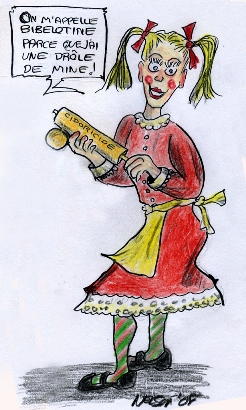
\includegraphics[height=60mm]{intro/preface/img/personnage-bibelotine.jpg}
\end{floatingfigure}

Évidemment, je suis journaliste pigiste, ce qui est un avantage réel par rapport au romancier de métier, un créateur isolé qui, comme le veut le cliché, applique avec rigueur la trame qu’il a imaginée et qui, durant le processus de création, limite l’interaction au minimum vital. C’est qu’avec le temps, le pigiste n’a plus d’ego; les éditeurs, rédacteurs en chef et autres chefs de pupitre le lui ont bouffé en totalité. Ainsi, que des lecteurs lui mettent publiquement sous le nez une «hénaurme» faute d’orthographe, une phrase boiteuse, une imprécision mortelle, une invraisemblance inopportune, ça ne l’affecte pas. Bien au contraire. Il s’en montre ravi, convaincu que son produit vient d’être amélioré. Qu’une lectrice ou un lecteur lui change un recoin d’histoire en y ajoutant une perspective amusante, il la fait sienne et se dépêche d’en donner le crédit à la si gentille personne.

Dans les pages qui suivent ce roman, vous trouverez mon analyse du processus encouru, une démarche que l’on dit de type «Web 2.0». Vous rencontrerez le chœur dont parle Simon, vous jugerez du sérieux de son apport, de sa générosité et de sa gentillesse. Vous saurez pourquoi, dans Le joueur de lyre, il ya des personnages qui se nomment Bea Bellow, Vlado Markovsky, Anton Suzkinne, Thierry-Ian Dennis-Dubeau, Louise Lavoie, Tropecolo, Philippe Flipper Dauphin, les Papyblues et autres docteurs Bellavance. Surtout, vous comprendrez mon envie de recommencer la même expérience avec une nouvelle histoire dès que ce sera possible.

En parallèle avec ce magnifique chœur, j’ai soumis mes interrogations, mes angoisses, mes incompréhensions, à une belle soliste, ma blonde Darisse, une personne d’une sensibilité prodigieuse qui a su me saupoudrer l’histoire de considérations humaines. Je lui dois notamment les réactions complexes du personnage de Marie-Odile Tremblay. Plus globalement, elle a, semaine après semaine, écouté mon récit du chapitre devant être mis en ligne et m’a régulièrement aidé à le solidifier. 

%\begin{floatingfigure}[l]{15mm}
%
\includegraphics[height=10mm]{intro/preface/img/druide1.jpg}
%\end{floatingfigure}

En terminant, un remerciement à André d’Orsonnens, PDG de Druide informatique, qui m’a gracieusement fourni un exemplaire d’Antidote, le coffret d’outils linguistiques bien connu. Dans le cas d’un pigiste devant mettre en ligne, tous les vendredis matin, un texte de quelque 7 000 mots se voulant un nouveau chapitre du Joueur de lyre, ce logiciel montréalais m’a fait gagner beaucoup de temps.

Voilà ! Bienvenu dans mon histoire et bonne lecture ! On se retrouve plus tard, pour la partie analyse.

Nelson Dumais, janvier 2009

